So izboljšani tip eno-vretenskih avtomatov. Imajo od
2 do 8 vreten ampak se večinoma uporabljajo 4 ali 6
vretenski avtomati. Cikel obdelovanja kosa se zaključi,
ko se revolver z obdelovanci obrne za 1 obrat. Na vsaki stopnji
obrata se izvede ena stopnja obdelave, kot je prikazano na
sliki \ref{vec_vretenc}, zato je skupni čas za en
kos enak eno-vretenskemu avtomatu, le produktivnost je veliko
večja. Čas ene stopnje obdelave je odvisna od časa najdaljše
obdelave na kosu. Npr. če imamo 5 postaj na katerih se struži 5s
in eno postajo na kateri se vrta 10s, se bo vreteno obrnilo vsakih 10s.
Njihova velika prednost je zelo hiter čas cikla, slabost pa,
da je za nastavitev takšega stroja potrebno veliko časa, znanja
in dragega orodja. Zato se takšni stroji največ uporabljajo za
izjemno velike serije, kjer se dela samo en izdelek in se stroj
ne nastavlja na nove kose.

\begin{figure}[H]
	\begin{center}
		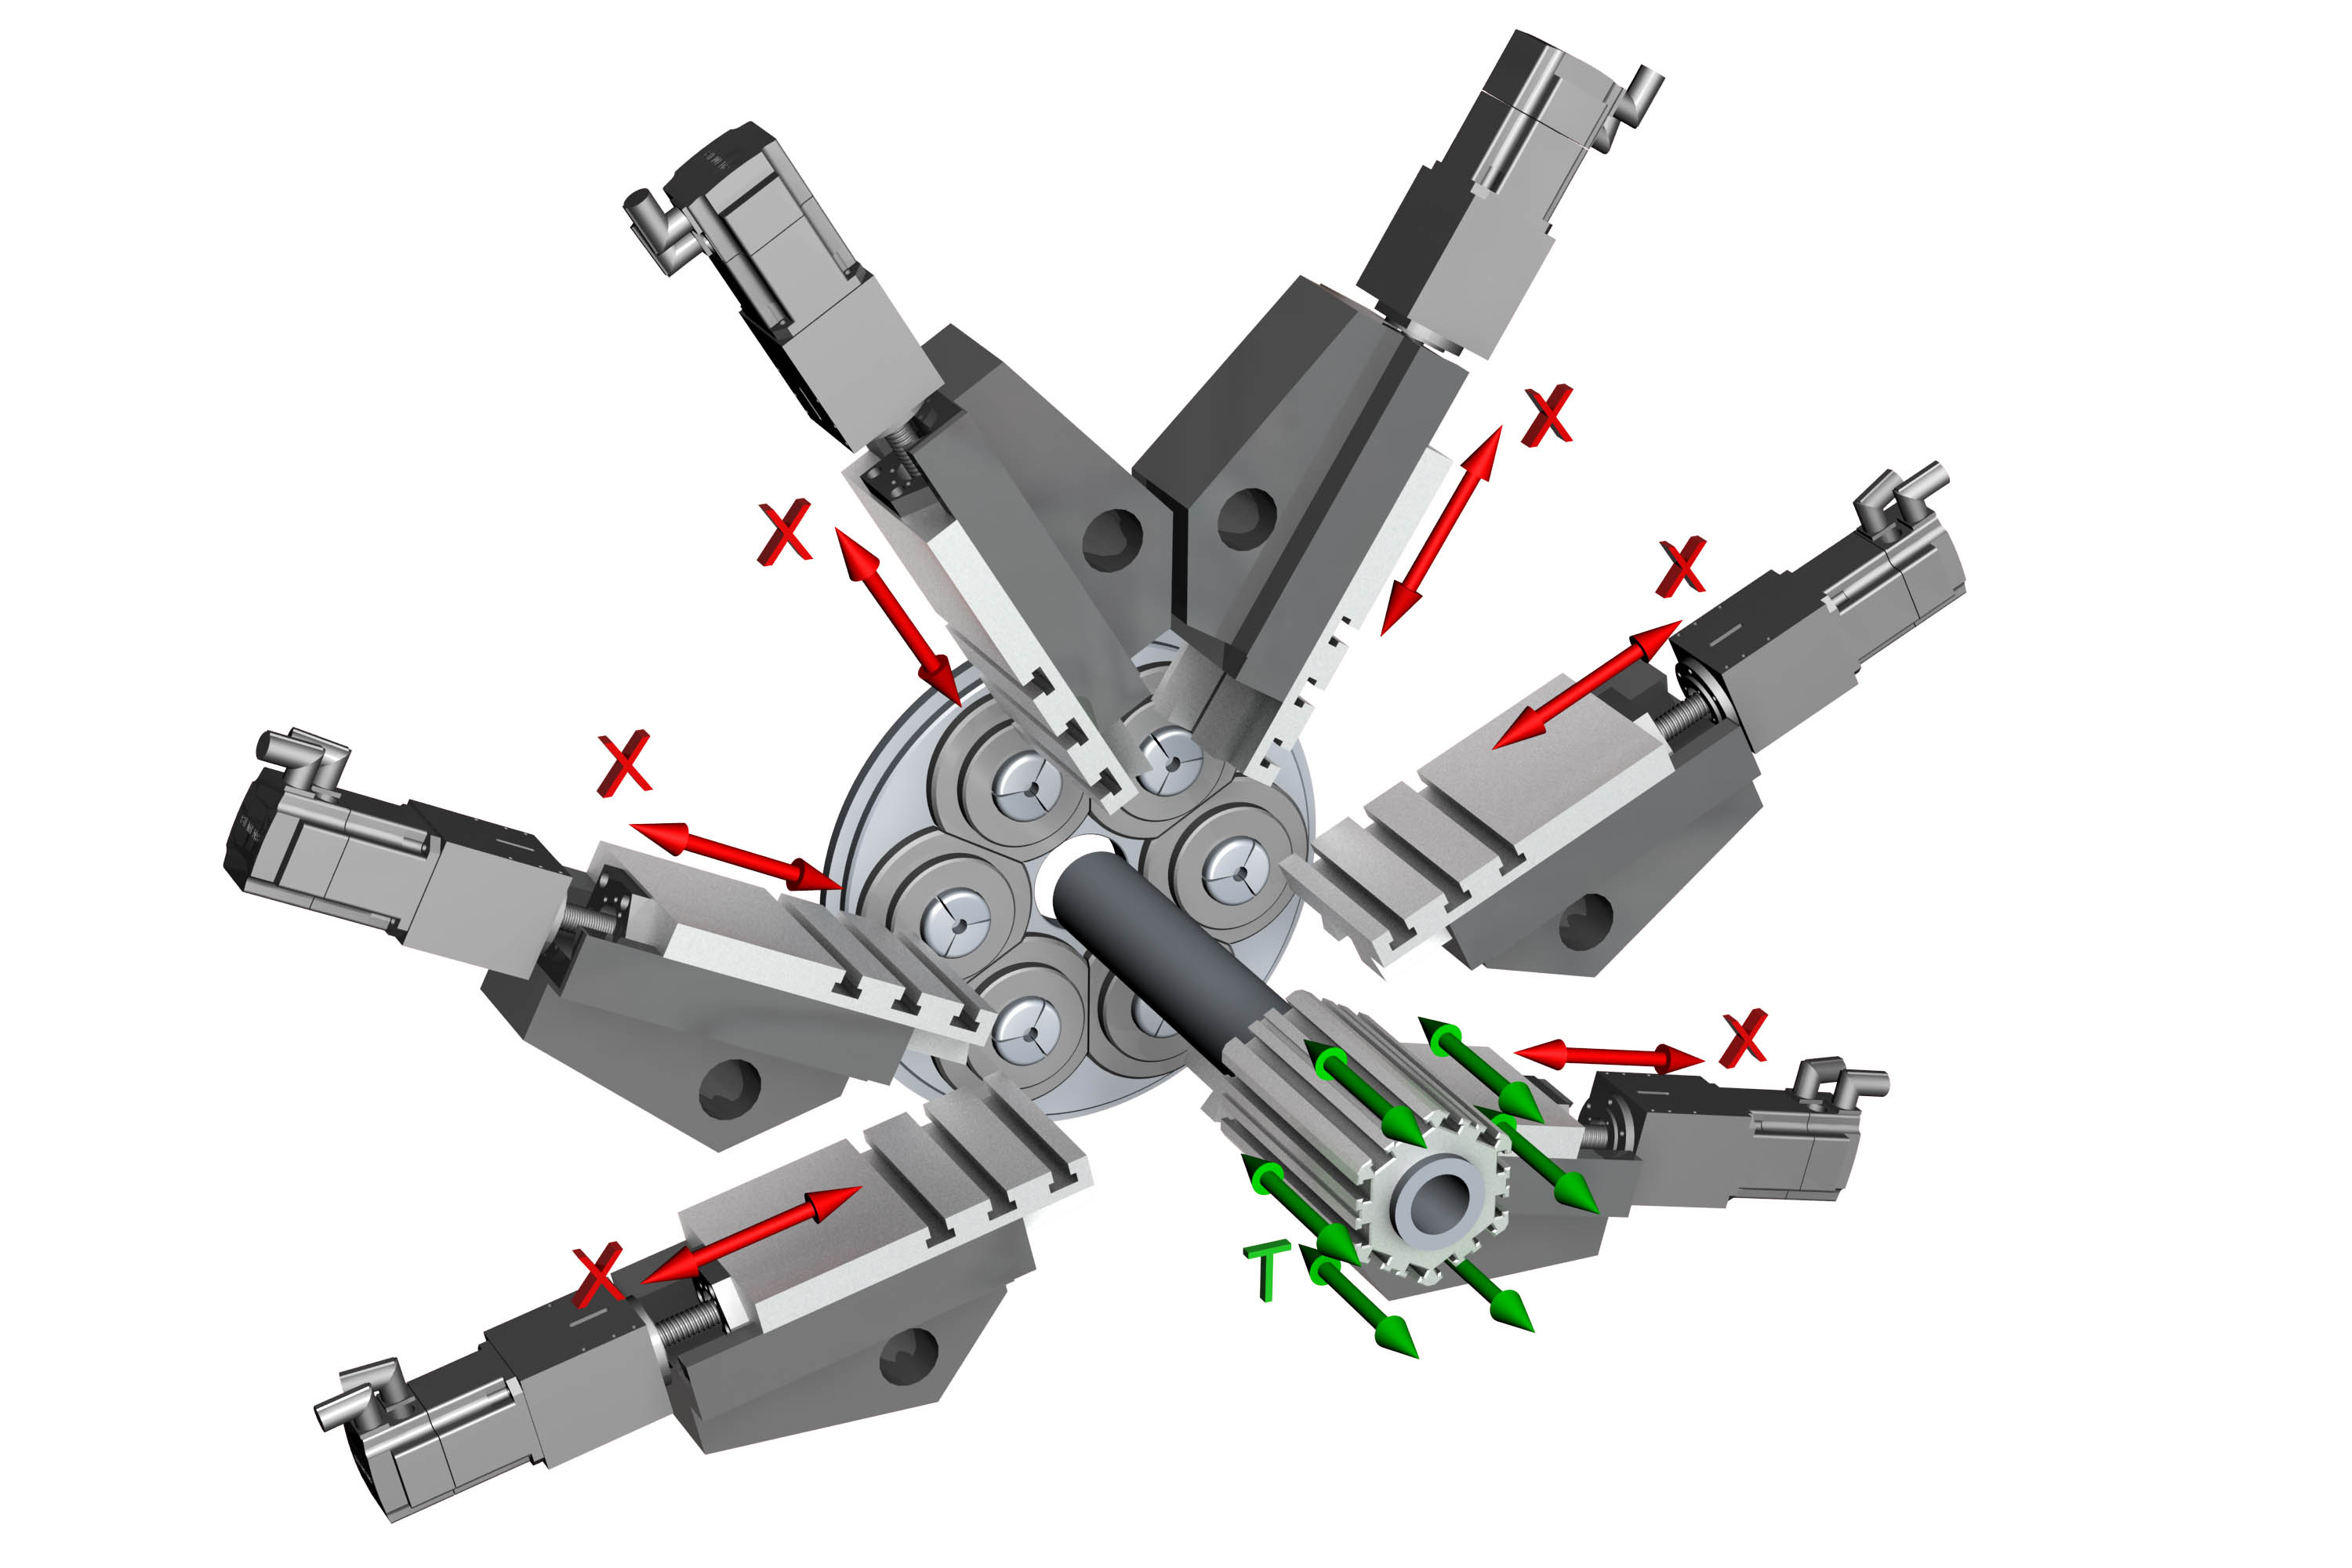
\includegraphics[width=\linewidth]{vec_vretenski_avtomat_shema.jpg}
		\caption{Shema več vretenskega avtomata
			\cite{vec_vretenska_struznica_shema}}
		\label{vec_vretenc}
	\end{center}
\end{figure}